\documentclass[11pt,a4paper]{article}
\usepackage{notes}

\title{Problem Set: Magnetic Methods}
\author{Geophysics 3A}
\date{}

\begin{document}
\maketitle

\section*{Question 1: Magnetic Anomalies of Simple Bodies\hfill [10 pts.]}

This question builds on \textbf{Week 5, Activity 2: Magnetic Structures}.

For each of the following bodies assume:
\begin{itemize}[itemsep=-0.5em]
    \item a uniform vertical inducing geomagnetic field with,
    \item constant magnetic susceptibility within each body,
    \item magnetization is purely induced (no remanent magnetization),
    \item the observed quantity is the vertical magnetic anomaly, $B_z$.
\end{itemize}

\subsection*{(A) Conceptual predictions}

\begin{figure}[h!]
\centering

% =========================
% Row 1
% =========================

\begin{minipage}[t]{0.48\textwidth}
\centering
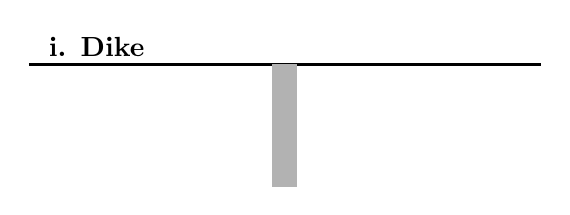
\begin{tikzpicture}[scale=0.65]
  \node[anchor=west,font=\bfseries] at (-4.8,0.35) {i. Dike};
  \draw[thick] (-5,0) -- (5,0);
  \fill[gray!60] (-0.25,0) rectangle (0.25,-2.4);
\end{tikzpicture}
\end{minipage}
\hfill
\begin{minipage}[t]{0.48\textwidth}
\centering
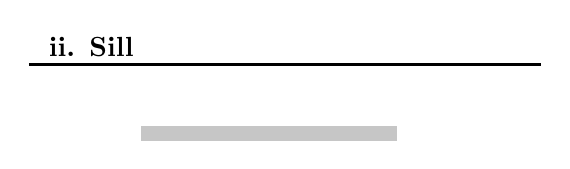
\begin{tikzpicture}[scale=0.65]
  \node[anchor=west,font=\bfseries] at (-4.8,0.35) {ii. Sill};
  \draw[thick] (-5,0) -- (5,0);
  \fill[gray!45] (-2.8,-1.2) rectangle (2.2,-1.5);
\end{tikzpicture}
\end{minipage}

\vspace{1em}

% =========================
% Row 2
% =========================

\begin{minipage}[t]{0.48\textwidth}
\centering
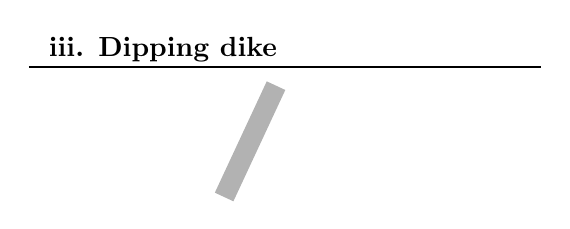
\begin{tikzpicture}[scale=0.65]
  \node[anchor=west,font=\bfseries] at (-4.8,0.35) {iii. Dipping dike};
  \draw[thick] (-5,0) -- (5,0);
  \begin{scope}[rotate=-25]
    \fill[gray!60] (-0.2,-0.4) rectangle (0.2,-2.8);
  \end{scope}
\end{tikzpicture}
\end{minipage}
\hfill
\begin{minipage}[t]{0.48\textwidth}
\centering
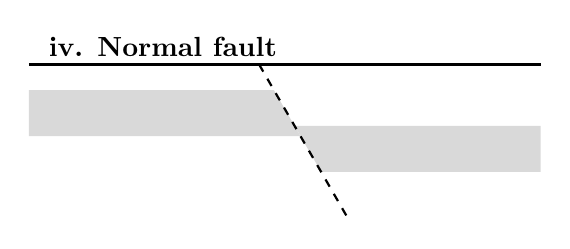
\begin{tikzpicture}[scale=0.65]
  \node[anchor=west,font=\bfseries] at (-4.8,0.35) {iv. Normal fault};

  \draw[thick] (-5,0) -- (5,0);

  \def\xf{-0.5}
  \def\dip{60}
  \def\tlay{0.9}
  \def\ztopL{-0.5}
  \def\ztopR{-1.2}

  \pgfmathsetmacro{\cosd}{cos(\dip)}
  \pgfmathsetmacro{\sind}{sin(\dip)}
  \pgfmathsetmacro{\cotd}{\cosd/\sind}

  \pgfmathsetmacro{\zLt}{\ztopL}
  \pgfmathsetmacro{\zLb}{\ztopL - \tlay}
  \pgfmathsetmacro{\xLt}{\xf - (\zLt)*\cotd}
  \pgfmathsetmacro{\xLb}{\xf - (\zLb)*\cotd}

  \pgfmathsetmacro{\zRt}{\ztopR}
  \pgfmathsetmacro{\zRb}{\ztopR - \tlay}
  \pgfmathsetmacro{\xRt}{\xf - (\zRt)*\cotd}
  \pgfmathsetmacro{\xRb}{\xf - (\zRb)*\cotd}

  \path[fill=gray!30,draw=none]
       (-5,\zLt) -- (\xLt,\zLt) -- (\xLb,\zLb) -- (-5,\zLb) -- cycle;

  \path[fill=gray!30,draw=none]
       (\xRt,\zRt) -- (5,\zRt) -- (5,\zRb) -- (\xRb,\zRb) -- cycle;

  \draw[dashed,thick] (\xf,0) -- ++({3.5*\cosd},{-3.5*\sind});
\end{tikzpicture}
\end{minipage}

\caption{Idealized 2-D susceptibility structures used to explore magnetic anomaly geometry.}
\end{figure}

For each geometry:
\begin{enumerate}
    \item Sketch the expected vertical magnetic anomaly as a function of horizontal distance.
    \item Indicate the locations of maxima and minima relative to the body.
    \item Comment on symmetry or asymmetry of the anomaly.
    \item Describe the far-field (long-wavelength) behavior.
    \item Compare qualitatively with the gravity anomaly for the same structure.
\end{enumerate}


\subsection*{(B) Forward modelling}

Using the Talwani magnetic modelling code (\verb+gravmag2d_gui.py+):

\begin{enumerate}[itemsep=-0.5em]
    \item Construct polygons corresponding to the bodies above.
    \item Assign a constant magnetic susceptibility contrast.
    \item Compute the vertical magnetic anomaly $B_z(x)$.
    \item Compare modelled anomalies to your sketches.
    \item For the vertical dike, investigate how burial depth, susceptibility contrast,
          body width, and field inclination affect anomaly wavelength and amplitude.
\end{enumerate}


\section*{Question 2: Dipole Anomalies \hfill [10 pts.]}

For a vertical magnetic dipole ($\hat{m} = \hat{z}$) the radial and azimuthal components of the magnetic field in spherical coordinates (from the notes) are
\begin{align*}
    B_r & = \frac{\mu_0}{2\pi} \frac{m \cos \theta}{r^3}, \\
    B_\theta & = \frac{\mu_0}{4\pi} \frac{m \sin \theta}{r^3}, \\
    B_\phi & = 0,
\end{align*}
where $r$ and $\theta$ are the distance to and the co-latitude of the dipole at a point $P$.  However, since we wish to know the vertical component of the field, we must convert the field to Cartesian coordinates from spherical.  The conversion of a vector in spherical, $B(r,\phi,\theta)$, to Cartesian coordinates, $B(x,y,z)$, is performed by 
\begin{equation*}
    \begin{bmatrix}
        B_x \\
        B_y \\
        B_z
    \end{bmatrix}
    =
    \begin{bmatrix}
        \sin \theta \cos \phi & \cos \theta \cos \phi & -\sin \phi \\
        \sin \theta \sin \phi & \cos \theta \sin \phi & \cos \phi \\
        \cos \theta           & -\sin \theta          & 0
    \end{bmatrix}
    \begin{bmatrix}
        B_r \\
        B_\theta \\
        B_\phi
    \end{bmatrix},
\end{equation*}
where
\begin{align*}
    r &= (x^2 + y^2 + z^2)^{1/2} \\
    \phi &= \tan^{-1} \frac{y}{x} \\
    \theta &= \cos^{-1} \frac{z}{r} =
        \sin^{-1} \frac{(x^2 + y^2)^{1/2}}{r}.
\end{align*}
Note that in for these problems, we can assume $y = 0$ and $\phi = 0$.
\begin{figure}[hbt]
  \centering
  \includegraphics[]{figures/vertical_dipole.eps}
  \caption{Vertical magnetic dipole with moment $m = 1$ at 1~m below the surface.}
  \label{fig:vdipole}
\end{figure}

\begin{enumerate}
    \item \label{itm:vdipole} Show that the vertical magnetic field due to a vertically oriented dipole is given by,
    \begin{equation}
        B_z = \frac{\mu_0}{4 \pi} \frac{m}{r^3}
            \left[ 3 \cos^2 \theta - 1 \right].
    \end{equation}
    Remember, $\cos^2 \theta + \sin^2 \theta = 1$.

    \item \label{itm:hdipole}If we wish to know the vertical field at the surface of the Earth due to a buried dipole with an arbitrary rotation of the dipole axis, $\hat{m}$, about $\hat{y}$.  We define the rotation angle, $\alpha$, such that
    \begin{equation*}
        \theta = \theta' + \alpha,
    \end{equation*}
    where $\theta$ is the angle between the $\hat{z}$ and $P$, $\theta'$ is the angle between the $\hat{m}$ and the point $P$, and $\alpha$ is the angle between $\hat{z}$ and $\hat{m}$.  In this case the magnetic field is given by
    \begin{align*}
        B_{r'} & = \frac{\mu_0}{2\pi} \frac{m \cos {\theta'}}{r^{3}}, \\
        B_{\theta'} & = \frac{\mu_0}{4\pi} \frac{m \sin {\theta'}}{r^{3}}.
    \end{align*}
    Note that $r' = r$ since the distance between the dipole and $P$ does not change under rotation.  The vertical field for a rotated dipole is
    \begin{align*}
        B_z & = B_{r'} \cos \theta - B_{\theta'} \sin \theta \\
            & = \frac{\mu_0}{4 \pi} \frac{m}{r^3} 
            \left[ 2 \cos \left(\theta - \alpha\right) \cos \theta 
            - \sin \left(\theta - \alpha\right) \sin \theta \right].
    \end{align*}
    \begin{figure}[hbt]
      \centering
      \includegraphics[]{figures/dipole_coords.eps}
      \caption{Coordinate system for a dipole with arbitrary rotation of the dipole axis, $\hat{m}$, by an angle $\alpha$ w.r.t.\ $\hat{z}$.}
      \label{fig:coords}
    \end{figure}

    Show that a horizontal dipole, $\alpha = \frac{\pi}{2}$, the vertical magnetic is therefore given by
    \begin{equation}
        B_z = \frac{3 \mu_0}{4 \pi} \frac{m}{r^3}
            \cos \theta \sin \theta . 
    \end{equation}
    Recall that $\cos \left(\theta - \frac{\pi}{2}\right) = \sin \theta$ and $\sin \left(\theta - \frac{\pi}{2}\right) = -\cos \theta$.  Note: this result is identical to $B_x$ for a vertical dipole.
    \begin{figure}[hbt]
      \centering
      \includegraphics[]{figures/horizontal_dipole.eps}
      \caption{Horizontal magnetic dipole with moment $m = 1$ at 1~m below the surface.}
      \label{fig:hdipole}
    \end{figure}

    \item Compute the vertical component of the magnetic field strength, $B_{z}$, at the surface of the Earth for a {\bf vertical} magnetic dipole buried a depth $z$ below the surface (Figure~\ref{fig:vdipole}).  Plot your result.  For your axes, plot the vertical axes in terms of factors of
    \begin{equation}
        M = \frac{\mu_0 m}{4 \pi z^3} .
    \end{equation}
    

    \item Compute the vertical component of the magnetic field strength, $B_{z}$, at the surface of the Earth for a {\bf horizontal} magnetic dipole buried a depth $z$ below the surface (Figure~\ref{fig:hdipole}).  Plot your result as above in terms of
    \begin{equation}
        M = \frac{\mu_0 m}{4 \pi z^3} .
    \end{equation}

    \item {\bf Anomaly width to depth relations} \\
    Estimating the depth to a structure based on the width or half-width of the anomaly is a useful field tool.  Using the equations for a vertical dipole, show that the depth of the dipole is approximately equal to its depth.  Start by equating the solution at $x=0$ to the solution at $x_{1/2}$.

    Note, you will have to solve a 10-th order polynomial to solve this problem.  You can use Wolfram Alpha online to solve for the polynomial.
    
    For a horizontal dipole, use the peak to peak width to develop a rule for the anomaly width to burial depth.  Remember to find the locations of the peaks you will have to minimize the function, i.e., $\dv{B_z}{x} = 0$ and solve for $x$.
        
    Check your result in relation to your graphical results from Problems~\ref{itm:vdipole} and \ref{itm:hdipole}.
\end{enumerate}


\section*{Question 3: Magnetic Susceptibility and Mineral Content\hfill [10 pts.]}

\begin{enumerate}[itemsep=-0.5em]
    \item Magnetite (mt) has a susceptibility of order $\chi_{\text{mt}}\approx1$--$5$.  Show that the bulk susceptibility of a rock can be approximated as
    \[
        \chi_{\text{bulk}} \approx f_{\text{mt}}\chi_{\text{mt}},
    \]
    where $f_{\text{mt}}$ is the volume fraction of magnetite.

    \item Estimate the magnetite volume fraction required to produce bulk susceptibilities of $10^{-3}$ and $10^{-2}$.

    \item Convert these to weight percent magnetite, assuming
    $\rho_{\text{mt}} = \SI{5200}{\du}$ and
    $\rho_{\text{rock}}= \SI{2700}{\du}$.

    \item Briefly discuss why magnetic anomalies are often dominated by small concentrations of magnetite.
\end{enumerate}


\section*{Question 4: Disappearance of Marine Magnetic Anomalies\hfill [10 pts.]}

Marine magnetic anomalies weaken near continental margins.

\begin{enumerate}[itemsep=-0.5em]
  \item Assume a linear geotherm
  \[
  T(z) = T_s + \frac{qz}{k},
  \]
  with $T_s = \SI{0}{\degC}$, $q = \SI{70}{\hfu}$, and $k = \SI{2.3}{\tcu}$. Stein \& Stein (1992) developed a plate cooling model for the oceans.  They suggest oceanic heat flow may be predicted as $q = 510\,t^{-1/2}$ where $t$ is the age of the seafloor in \si{Ma} and heat flow is in \si{\hfu}.

  Estimate the depth to the Curie temperature of magnetite
  ($T_C \approx \SI{150}{\degC}$) as a function of age.

  \item Determine the thickness of sediment required such that the top of the basaltic basement exceeds the Curie temperature, assuming a thermal conductivity of \SI{1.5}{\tcu}.

  \item Explain how sediment accumulation, elevated temperatures, and increased depth combine to suppress marine magnetic anomalies near continental margins.
\end{enumerate}

\end{document}